\documentclass[a4paper,11pt]{report}
\usepackage[italian]{babel}
\usepackage[utf8]{inputenc}
\usepackage[total={170mm,267mm},top=15mm,bottom=15mm,left=21mm,right=21mm]{geometry}
\usepackage{graphicx}

\begin{document}

\begin{titlepage}
  \clearpage\thispagestyle{empty}
  \centering
  \vspace{1cm}
  {\normalsize Informatica - Area scientifica \\  Dipartimento di Scienze matematiche, informatiche e multimediali\\  Università di Udine \par}
  \vspace{3cm}
  {\Huge \textbf{Progetto di Social Computing \newline
  } \LARGE{Crowdsorcing con Crowd Frame  parte 1}
  }

  \vspace{4cm}
  {\Large  Parata Loris (144338) \\ Arzon Francesco (142439)\\ Dal Fabbro Lorenzo (142300)\\ }
  \vspace{12cm}
  {\normalsize Anno accademico 2020/2021}
  \pagebreak
\end{titlepage}

\tableofcontents{}
\pagebreak
\chapter{Crowd Frame}
\section{Introduzione}
Questo secondo progetto di Social Computing si suddivide in due parti, la fase di progettazione di un task di crowdsourcing e la fase di raccolta dati e analisi dei dati ottenuti da un piccolo gruppo di workers.
In questa relazione si documenta  la prima parte dell'esperimento di crowdsourcing, la progettazione del task richiesto dalla traccia.


\section{Progettazione del task}

\subsection{Obiettivo del task}
La traccia richiede di creare sei HIT differenti riguardanti tre libri, per ognuno dei quali si devono individuare tre edizioni differenti. Ogni HIT contiene tre edizioni, una per ogni libro di riferimento, per le quali ogni worker deve rispondere a 6 dimensioni differenti, quattro imposte dalla traccia e due scelte dal gruppo di progetto.
\subsubsection{Lingua del task}
Abbiamo deciso di sviluppare l'intero progetto in lingua inglese, in modo da rendere il progetto il più realistico e simile ai task presenti sulla piattaforma di crowdsourcing di MTurk. Di conseguenza abbiamo scelto dei libri le cui edizioni sono scritte in lingua inglese.

\subsection{Creazione del task}
La creazione del task è stata effettuata mediante l'utilizzo dell'interfaccia grafica del framework \textbf{Crowd Frame} per la semplicità con cui si presenta la GUI, anche se sono stati riscontrati alcuni problemi riguardanti la visualizzazione delle dimensioni che presentavano l'opzione "giustificazione". Problematiche che sono state corrette andando ad effettuare delle modifiche nel json delle dimensioni. 

%\begin{figure}[h]
%	\centering
%	\includegraphics[width=0.8\linewidth]{Relazione/Relazione/api_show_friendships}
%	\label{fig:apishowfriendships}
%\end{figure}

\subsection{Le istruzioni inerenti al task}
Le istruzioni... 


\begin{figure}[h]
	\centering
	\label{fig:followers}
\end{figure}

\pagebreak
\subsection{Questionario}
Il questionario è composto da sei questionari standard che sono i seguenti:
\begin{itemize}
	\item How much time do you usually spend reading?
	\item How many books do you usually read during the year?
	\item What's your favorite literary genre?
	\item Do you prefer books in the original language or translated?
	\item What format do you buy most of your books in?
	\item Where do you usually find yourself reading?
	\item Based on what you choose a book to buy?
\end{itemize}
In modo da poter stabilire il background letterario del worker, le sue abitudini nell'acquisto di un libro, in modo da poterne stabilire la qualità dello stesso.

\subsection{Le dimensioni}
Oltre alle quattro dimensioni imposte dalla traccia:
\begin{itemize}
	\item \textbf{Dimensione 1}: Would you buy this book?
	\item \textbf{Dimensione 2}: Does the price seem adequate to you?
	\item \textbf{Dimensione 3}: Indicate how adequate it seems to you
	\item \textbf{Dimensione 4}: What is your impression of this edition?
\end{itemize}
Abbiamo deciso di aggiungere :
\begin{itemize}
	\item \textbf{Dimensione 5}: If you've read any edition of this book, indicate a URL to identify it
	\item \textbf{Dimensione 6}: Select the option that indicates how much you agree with the following statement: \\ "I would recommend this edition to another person"
\end{itemize}
\subsubsection{Dimensione 5}
La dimensione 5 è stata introdotta per verificare se il worker abbia letto una qualsiasi edizione del libro ed eventualmente individuarne delle versioni alternative preferite dai workers. Nella situazione in cui un worker non abbia mai letto quel libro si possono valutare diversamente la qualità delle risposte.   
\subsubsection{Dimensione 6}
La dimensione 6 è stata introdotta per verificarne la coerenza con la risposta della dimensione  1, in modo da avere un minimo di controllo di qualità senza l'utilizzo delle gold question. L'utilizzo di questo strumento non è stato richiesto dalla traccia, ed essendo non ancora implementato nella GUI il controllo delle gold questions, era necessario modificare il codice del framework. La verifica di coerenza verrà effettuata nella fase di analisi.


\subsection{Struttura della HIT}
Ogni HIT è composta da : 
\begin{itemize}
	\item \textbf{id}: per identificare la versione del libro
	\item \textbf{title}: indica il titolo del libro
	\item \textbf{author}: indica l'autore/ gli autori del libro
	\item \textbf{number of pages}: indica il numero di pagine di cui è composto il libro
	\item \textbf{editor}: indica l'editore che ha pubblicato il libro
	\item \textbf{url}: contiene l'URL che fa riferimento all'immagine della copertina del libro
	\item \textbf{year of publication}: anno di pubblicazione dell'edizione di riferimento
\end{itemize}
che vengono visualizzati al worker.
 \pagebreak
\subsection{Modifiche al file HTML}
All'interno del file HTML tra le righe 200 e 223 abbiamo inserito il seguente codice: \\
\begin{figure}[h]
	\centering
	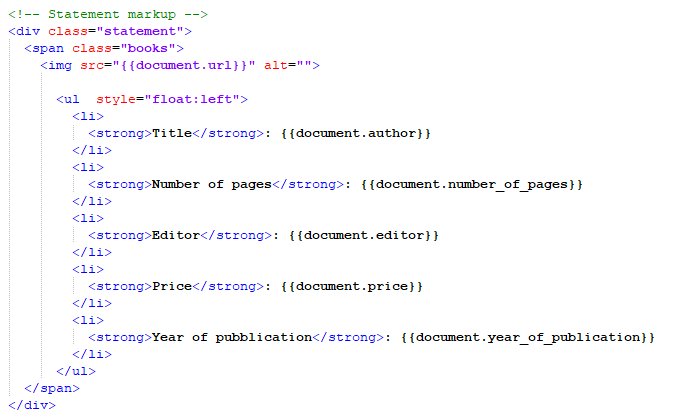
\includegraphics[width=0.9\linewidth]{statement}
	\label{fig:statement}
\end{figure}
In modo da visualizzare a sinistra l'immagine ed a destra gli attributi che descrivono il libro.

Inoltre è stata aggiunta una classe CSS nel file \textbf{skeleton.component.scss} in modo da poter rendere responsive l'immagine visualizzata della copertina del libro
\begin{figure}[h]
	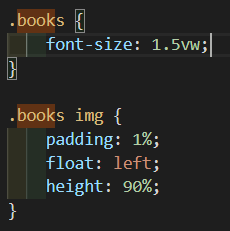
\includegraphics[width=0.3\linewidth]{css}
	\label{fig:css}
\end{figure}

\end{document}